%==================================
% (c) Jan Tulak, 2017
%%%%%%%%%%%%%%%%%%%%%%%%%%%%%%%%%%%%%%%%%%%%%%%%%%%%%%%%%%%%%%%%%%%%%%%%%%%%%

\chapter{XFS filesystem} \label{chap:xfs}
%----------------------------------------------------------------------

XFS is a journaling filesystem created by SGI in 1993. The new filesystem, intended as a powerful replacement of EFS with the expectation of growing amount of data in the future was first released in IRIX 5.3. Linux port began in 1999 and since 2002 is XFS accessible in the mainline Linux Kernel~\cite[Chap. 1.2, 1.3]{xfsHistory}.

\begin{table}[h]
\begin{tabular}{|l||r|r|r|r|}
\hline
& ext3 & ext4 & XFS & NTFS \\

\hline
\hline
max fs size & $16$ TiB & $16$ TiB & $16$ EiB& $256$ TiB\\
\hline
max file size & $8$ TiB & $16$ TiB & $8$ EiB & $256$ TiB\\
\hline
max files & $2^{32}$ & $2^{32}$& $2^{64}$ & $2^{32}$\\
\hline
date resolution & $1$ s & $1$ ns & $1$ ns & $100$ ns\\
\hline
\end{tabular}
\caption{Comparison of various filesystems and their limits. Sources:~\cite{inodesInLinux,NTFS1,NTFS2,NTFSfiletime,XFSforLinux}.}
\label{tab:xfs:comparison}
\end{table}



Because of its capabilities, XFS used also by well known institutions like CERN or Fermilab~\cite{XFSforLinux} for storing large amounts of data. Unlike most of other Linux filesystems, XFS is a 64bit fs, meaning it provides far greater limits for storage and file size\footnote{At least matured ones. Newer filesystems, like Btrfs, are also 64bit, but have not yet reached stability required in business sector.}, but its architecture also offer great scalability in terms of parallel I/O.

XFS as a whole is separated into three main projects: First, there is the XFS filesystem itself, in the form of a kernel module. Then a set of tools in a package called xfsprogs is tightly connected with XFS filesystem and contains programs useful or necessary for creation and manipulation of the filesystem. Among the tools included are {\tt mkfs.xfs}, on which this thesis is focused, but also other tools: {\tt fsck.xfs}, {\tt xfs\_io}, {\tt xfs\_growfs}, et cetera. And finally, there are xfstests, which is a test suite containing hundreds of shell scripts that verifying the behaviour of entire XFS chain (from mkfs to the kernel code). This project is also partially used by other filesystems. There are among others tests for ext4, overlay fs and btrfs.

Except for the xfstests test suite, xfsprogs also uses an automatical static analysis from Coverity~\cite{CoverityXfsprogs}. However, to see detailed information and defects there, one must be approved by existing members of the project.


%======================================================================
\section{XFS Architecture overview}\label{chap:xfs:overview}
%----------------------------------------------------------------------

When a XFS partition is formated, up to three areas are created on the disk: Data section is always present. An optional real-time section is omitted by default. Log section has to exist always but can be placed on a different device. The data part is then in fact split into multiple de facto independent filesystems called Allocation Groups, that handle space allocation and allows for higher parallelism, as most operations can be done on each Allocation Group independently on the others. The log section can be also internal to each of the Allocation Groups.

As each Allocation Group is a de facto standalone filesystem, each contains
the superblock and block and inode allocations and the only global
information, maintained by the first (primary) AG is free space and total
inode counts across the whole filesystem as can be seen
on figure~\ref{fig:xfs:primaryAG}.

\begin{figure}
  \centering
 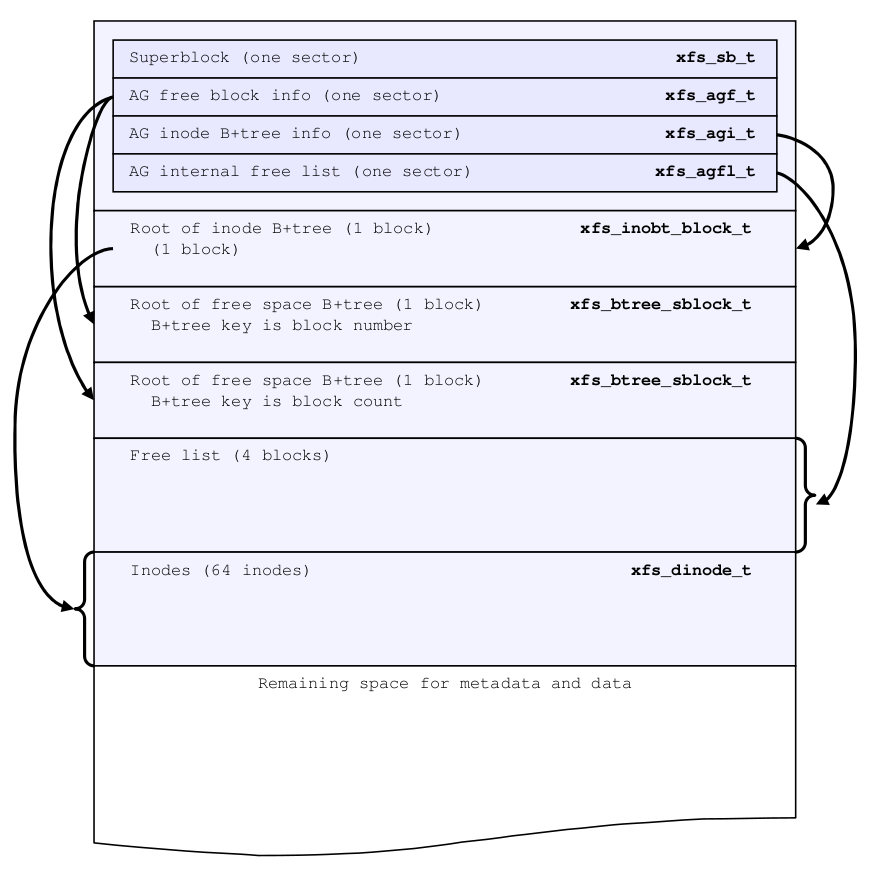
\includegraphics[width=13cm,keepaspectratio]{fig/primary-ag} % Or .pdf
 \caption{Primary AG right after mkfs~\cite[Ch. 3]{xfsStructure}.}
\label{fig:xfs:primaryAG}
\end{figure}
	
Real-time section is dedicated for files with a real-time attribute bit set, and operations with these files should have predictable latencies~\cite{xfsRealtime}. Log section is used to recover from situations like power failure on the next mount~\cite{xfsStructure,xfsman}.

When created on striped RAID\footnote{Striped RAID is e.g. RAID 0, where logically sequential data are split into a number of physical blocks and written on multiple disks interleaved. For a RAID 0 on two drives it means that odd blocks are located on one drive and even blocks on the other.}, XFS can be informed about it and align all allocations and size to the stripe unit to maximize speed.

As a native Unix filesystem, XFS uses {\em inodes} as a data structure to save information about files and directories. The first of the three parts of an inode (see figure~\ref{fig:xfs:inode}), core, contains the basic information, describing what the inode represents. Some example of the data in this field is the id of the user and group owning this inode, size and modification time.

\begin{figure}
  \centering
 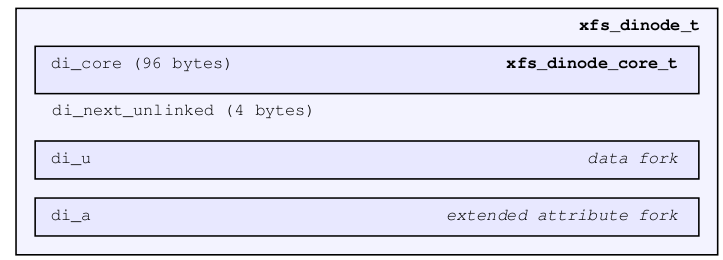
\includegraphics[width=12cm,keepaspectratio]{fig/inode} % Or .pdf
 \caption{On-disk inode~\cite[Ch. 4]{xfsStructure}.}
\label{fig:xfs:inode}
\end{figure}

The second part, {\tt di\_u}, or data fork, is for data for any specific type the inode can be; a directory, a symbolic link, a regular file, etc. For a directory, it will contain the entries in the directory. And the third member of each inode, {\tt di\_a}, is reserved for extended attributes (abbreviated {\tt xattr}), which are used for example by SELinux.

%======================================================================
\section{mkfs.xfs}\label{chap:xfs:mkfs}
%----------------------------------------------------------------------

This chapter describes in a greater detail the mkfs.xfs program itself, located
in file {\tt mkfs/mkfs\_xfs.c}, from user point of view. For information about
its implementation, see chapter~\ref{chap:refactoring:initialcodebase}. This
tool creates a new XFS filesystem with given properties. It is, as is usual for
core Unix utilities, a non-interactive program which accepts multiple arguments
when called and prints out the properties of the newly created filesystem if
successful, or prints an error and usage help when an error occurs.

\begin{lstlisting}[frame=none, basicstyle=\footnotesize\ttfamily, language=Bash, numbers=none, numberstyle=\tiny\color{black},caption= {Synopsis of mkfs.xfs utility~\cite{mkfs.xfsMan}.}]
mkfs.xfs [ -b block_size ] [ -d data_section_options ] [ -f ]
         [ -i inode_options ] [ -l log_section_options ] [ -n naming_options ]
         [ -p protofile ] [ -q ] [ -r real-time_section_options ]
         [ -s sector_size ] [ -L label ] [ -N ] [ -K ] device
\end{lstlisting}

An example of such usage is {\tt mkfs.xfs -f /dev/sda1}. This simple example creates a XFS filesystem on device {\tt /dev/sda1} even if an existing filesystem existed there -- thus the {\tt -f} (as force) flag. For the whole description of mkfs.xfs usage it is better to refer to mkfs.xfs manual page. What is important to note here is that parsing the input arguments and computing inner values based on these inputs makes most of the circa 3,500\footnote{Before the merge of the last part of my changes. With these changes, mkfs has over 4,000 lines.} lines of code.


%======================================================================
\section{xfstests}\label{chap:xfs:xfstests}
%----------------------------------------------------------------------

The project named {\em xfstests}, or also FSQA, is a framework and a
collection of test suites written in Bash. Most of the tests run some
filesystem utilities and either validates whether some part of the FS
ecosystem behaves correctly, or tries to replicate a specific known issue
to prevent regressions.

The tests are grouped into multiple categories according to the tested filesystem:

{\tt btrfs, cifs, ext4, f2fs, generic, ocfs2, overlay, shared, udf, xfs}

A grouping orthogonal to these categories assigns each test into one or
more groups that allows for finer tuning of which tests should be
run\footnote{An example of the groups: {\tt mkfs, quick, all, dangerous,
auto, quota, attr, symlink, \ldots}.}

These tests do not analyse any program (either its source code, or the
compiled binary), but only the results of running these programs, be it a
created filesystem, or printed messages. Because xfstests do not employ any
formal techninque and focus on completely different means of testing, it is
not compared with other tools in this work.
